\subsubsection{TCGA's RNAseq and mutations}


The Parsimonious Gene Correlation Analysis Network Analysis (PGCNA) was used to stratify breast, colon, and glioblastoma cancers \cite{Care2019-ij,Tanner2023-wa} based on gene expression. With the goal to better inform the MIBC subtyping, in this section we developed an integrative network approach to stratify MIBC. Our model differs from PGCNA by building the network using both gene expression and mutation as well as  domain knowledge through Transcription Factors (TFs).

% Weight modifiers 
The network weights are modified to integrated the mutation burden across the TCGA cohort into the network. At the network construction stage, after the Spearman correlation network and before the edge pruning the correlation values are changed according two opposing strategies. The reward strategy '\textit{promotes}' the genes which are highly mutated across tumour by increasing their weight, conversely the penalised strategy \textit{punishes} the genes that are highly mutated. The two modifiers are described in Figure \ref{fig:N_I:modifiers} where the highest mutated genes (e.g. TP53, TTN) are the most penalised/rewarded, while the weight values for un-mutated genes remain unchanged. It is worth mentioning, that there is no need to adapt the ModCon as the weight changes will affect the connectivity parameters from Equation \ref{eq:modcon}.

\begin{figure}[!htb]    \centering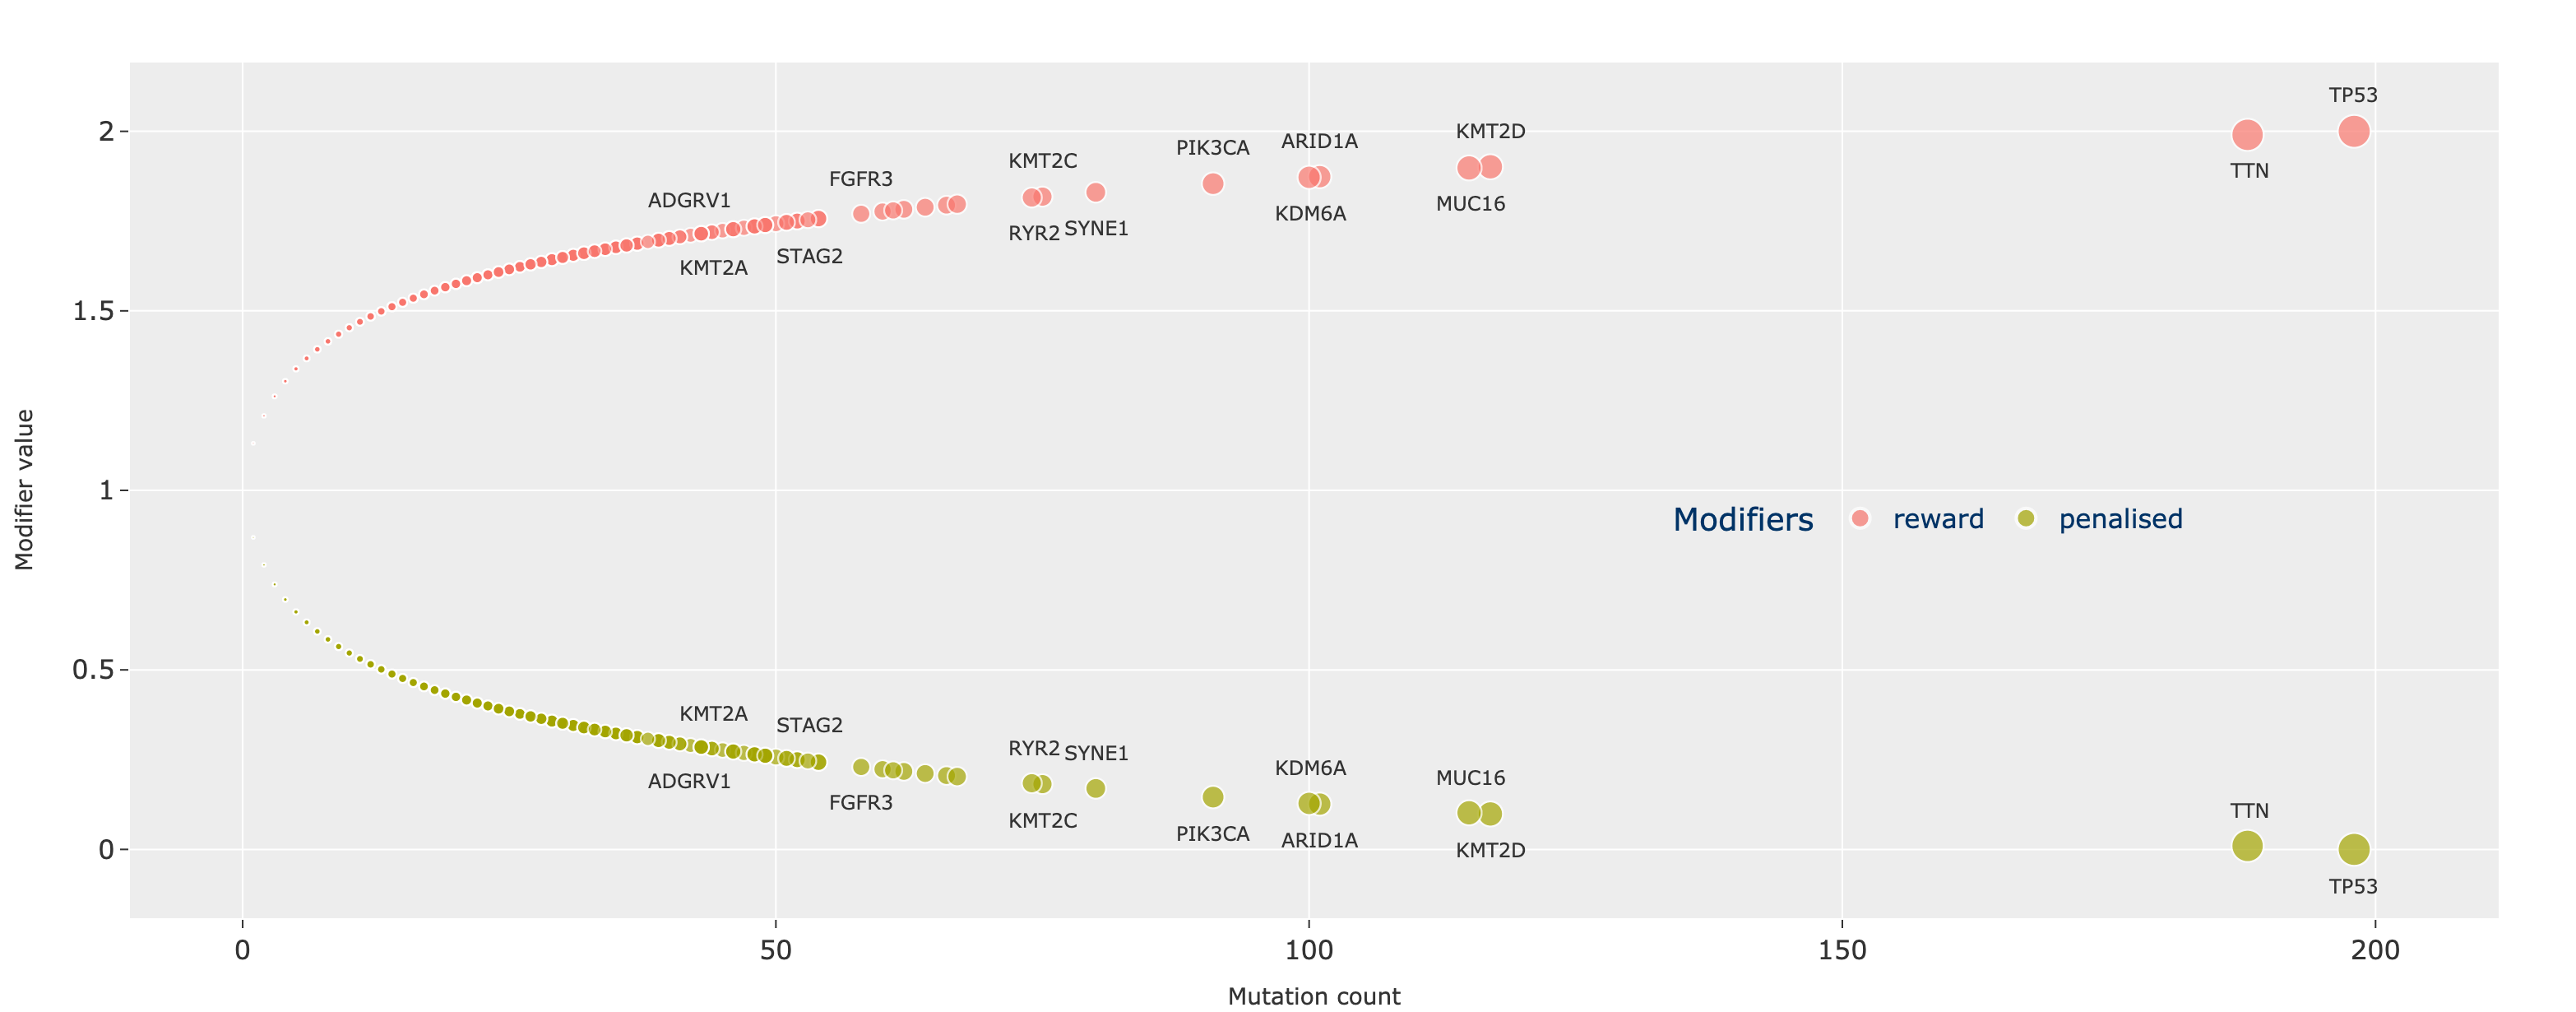
\includegraphics[width=0.9\textwidth,height=0.9\textheight,keepaspectratio]{Sections/Network_I/Resources/Methods/modifiers.png}
    \caption{Representing the two weight modifier strategies employed at the network construction stage. The blue, reward strategy, awards the genes that have a high burden across the cohort. Conversely, the  penalised strategy decreases the edges' strength for highly mutated genes. In both cases, the un-mutated genes remain unchanged.}
    \label{fig:N_I:modifiers}
\end{figure}


The node degree represents the number of connections a node has, a higher number, the more important the node is to the network. However, it is not only important how many connections there are but also to which nodes are these connections too, and PageRank\cite{Brin1998-mc} accounts for that. Thus, degree and PageRank are used in this project to described the network's centrality. It is also important how close the nodes are and if a node is an intermediate between others, thus the closeness and betweeness metrics are employed to describe the network. In addition, the Integrated Value of Influence (IVI) \cite{Salavaty2020-wo} combines multiple metrics and it is used to score the nodes have both a local and global influence to the network.

\begin{figure}[!htb]    \centering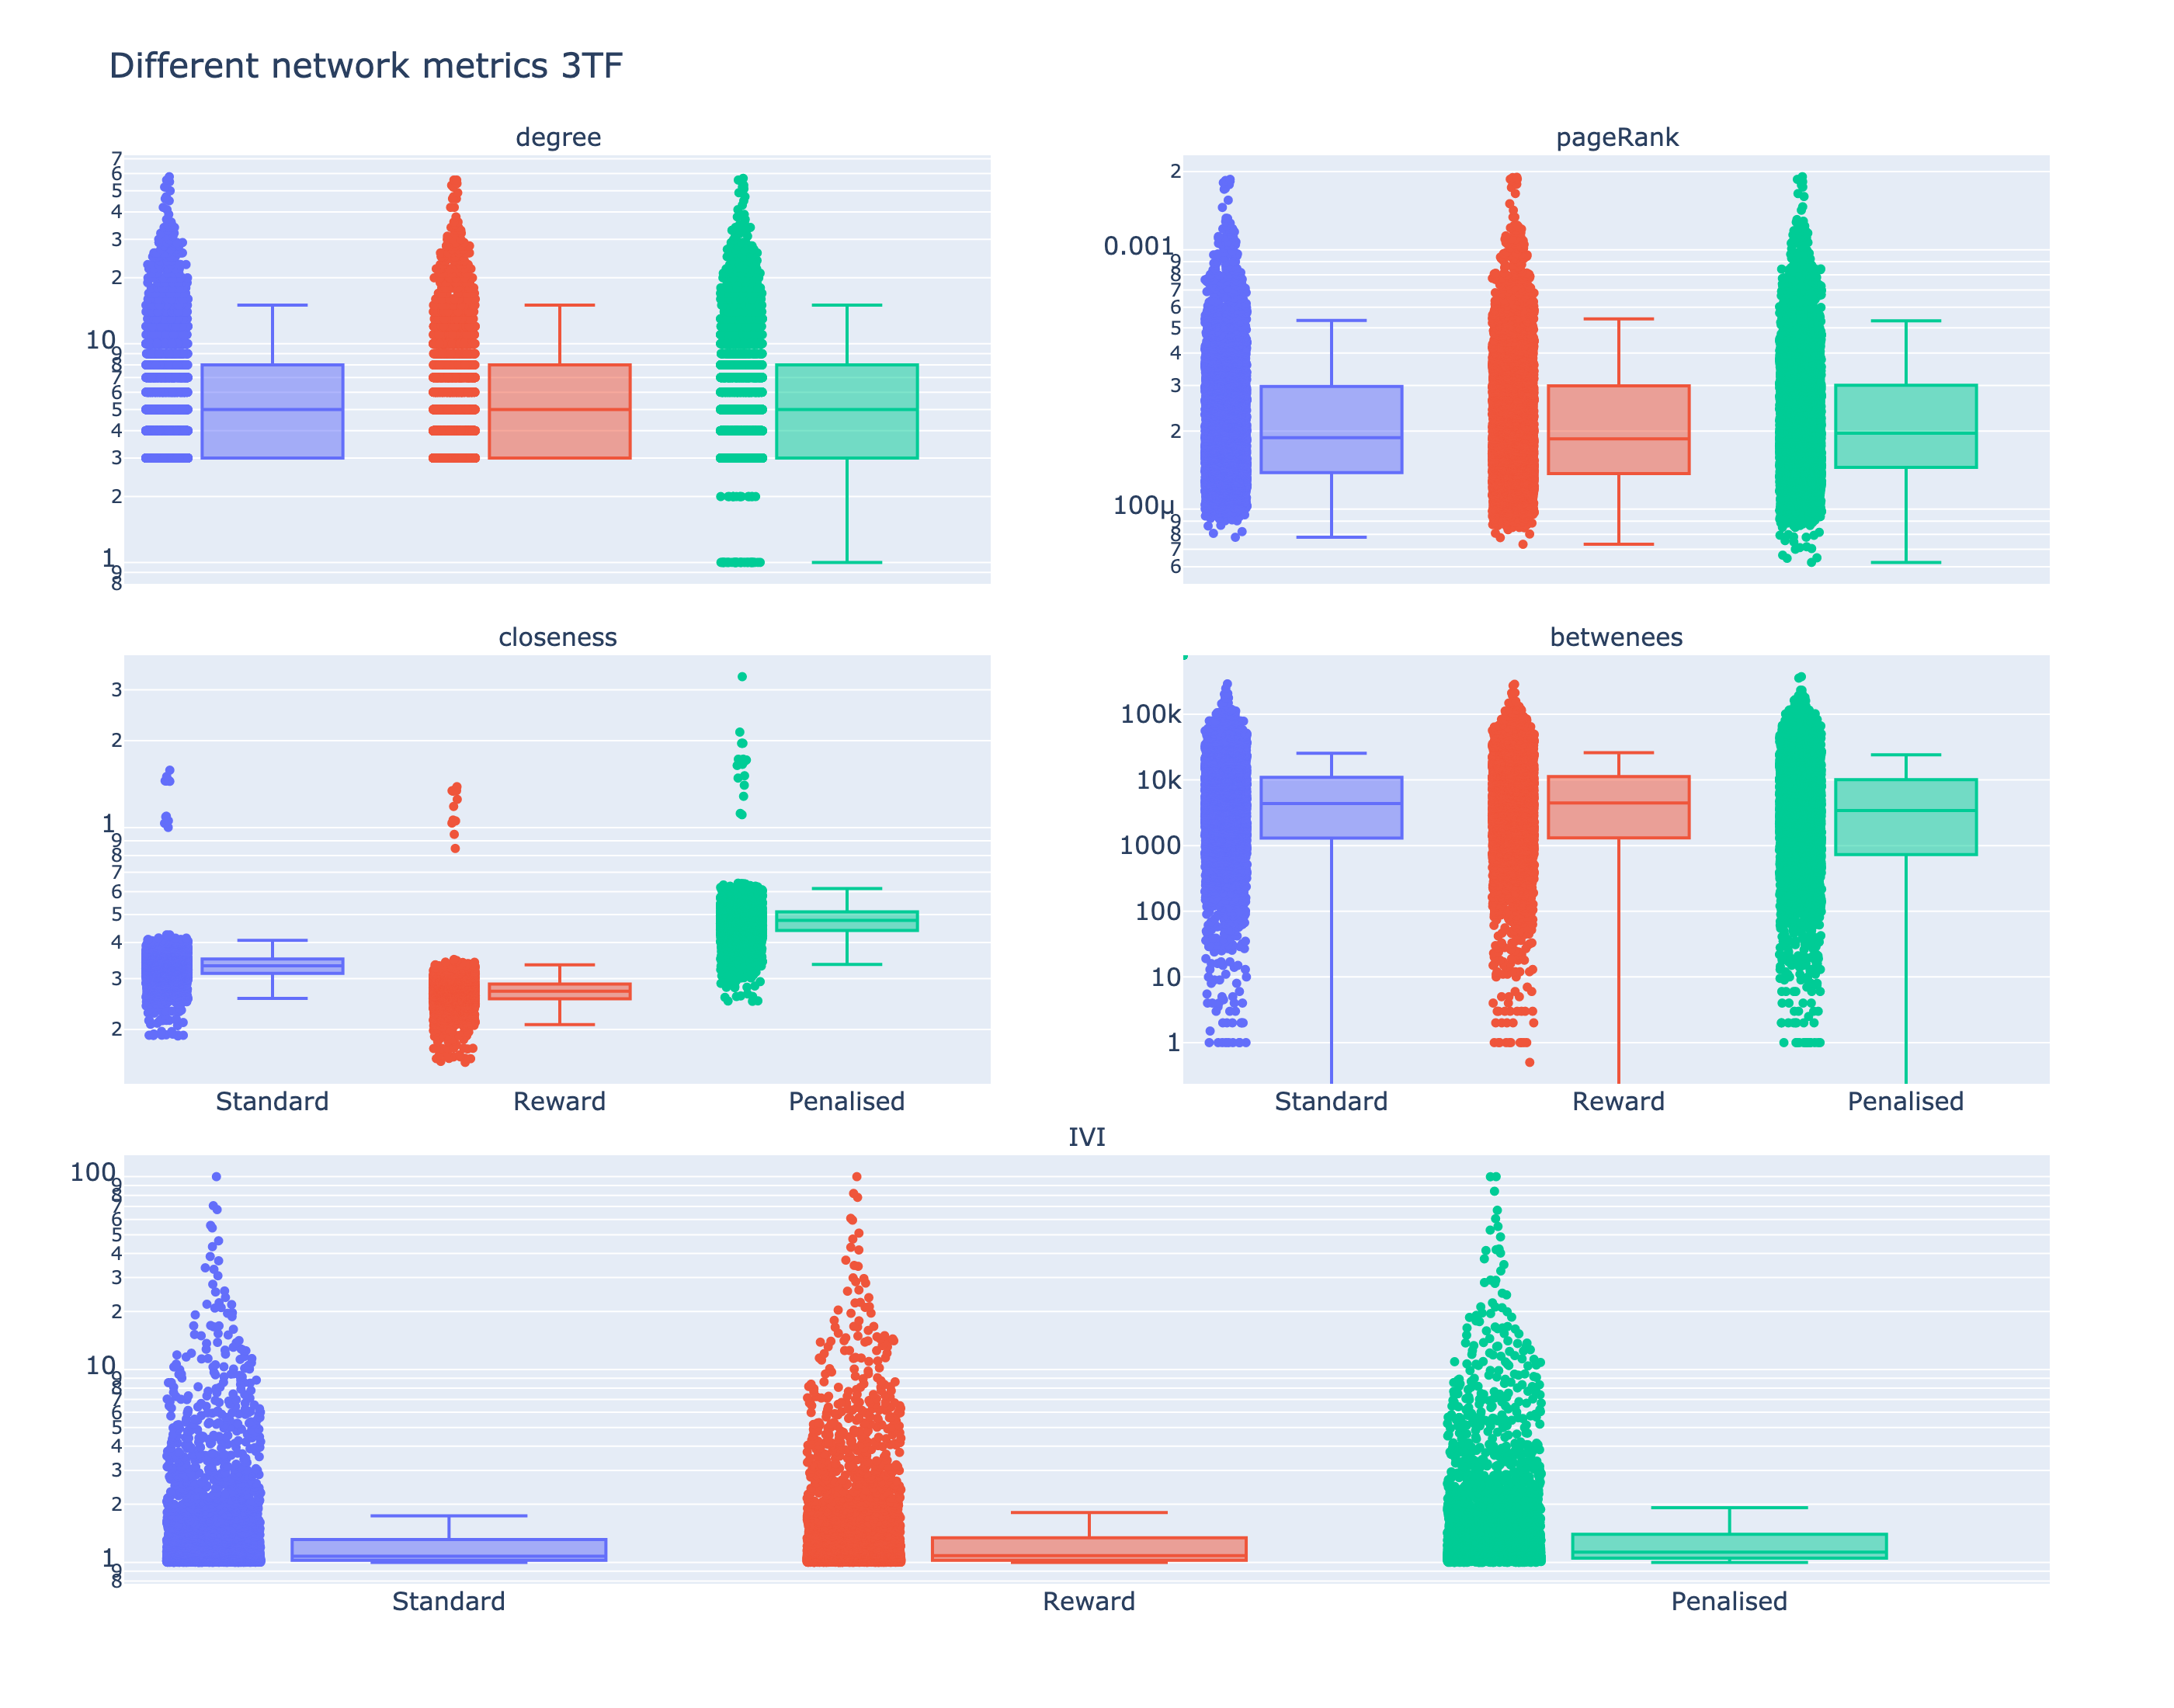
\includegraphics[width=1.0\textwidth,height=0.7\textheight,keepaspectratio]{Sections/Network_I/Resources/Tum_network/NetworkMetricsComp_10TF.png}
    \caption{Network metrics for the tumour networks formed from 4K genes, 3 connections per standard gene and 10 for TFs with the different weight modifiers; standard (blue), reward (red) and penalised (green). The y-axis represent the log10 of the meric. }
    \label{fig:N_I:net_metrics_tum}
\end{figure}

The different network metrics for standard (blue), reward (red) and penalised (green) are shown in Figure \ref{fig:N_I:net_metrics_tum}. The network metrics are generally similar across the different type modifiers with the exception of the penalised network where the nodes' degree is negatively affected and the the nodes are usually closer to each other (higher closeness values). This is due to the penalised function which almost prunes the connections for the highly mutated genes.

There are $\approx30K$ genes in the TCGA's MIBC cohort, from which less than a half ($\approx13K$) are considered expressed; more than 3 samples have TPM values larger than 0.5. From the $\approx13K$ genes there are $\approx10K$ genes which are mutated at least once are mutated, but then as the mutation burden is increased there are less genes represented as seen in Figure \ref{fig:N_I:mut_rep_tum}. The same trend can be noticed for TFs genes initially being 1027 genes in all the expressed genes, but only a few are mutated. The striking aspect of the Figure \ref{fig:N_I:mut_rep_tum} is the steep decrease of the genes mutated, we have explored different genes selection strategies in Section \ref{}.

\begin{figure}[!htb]    \centering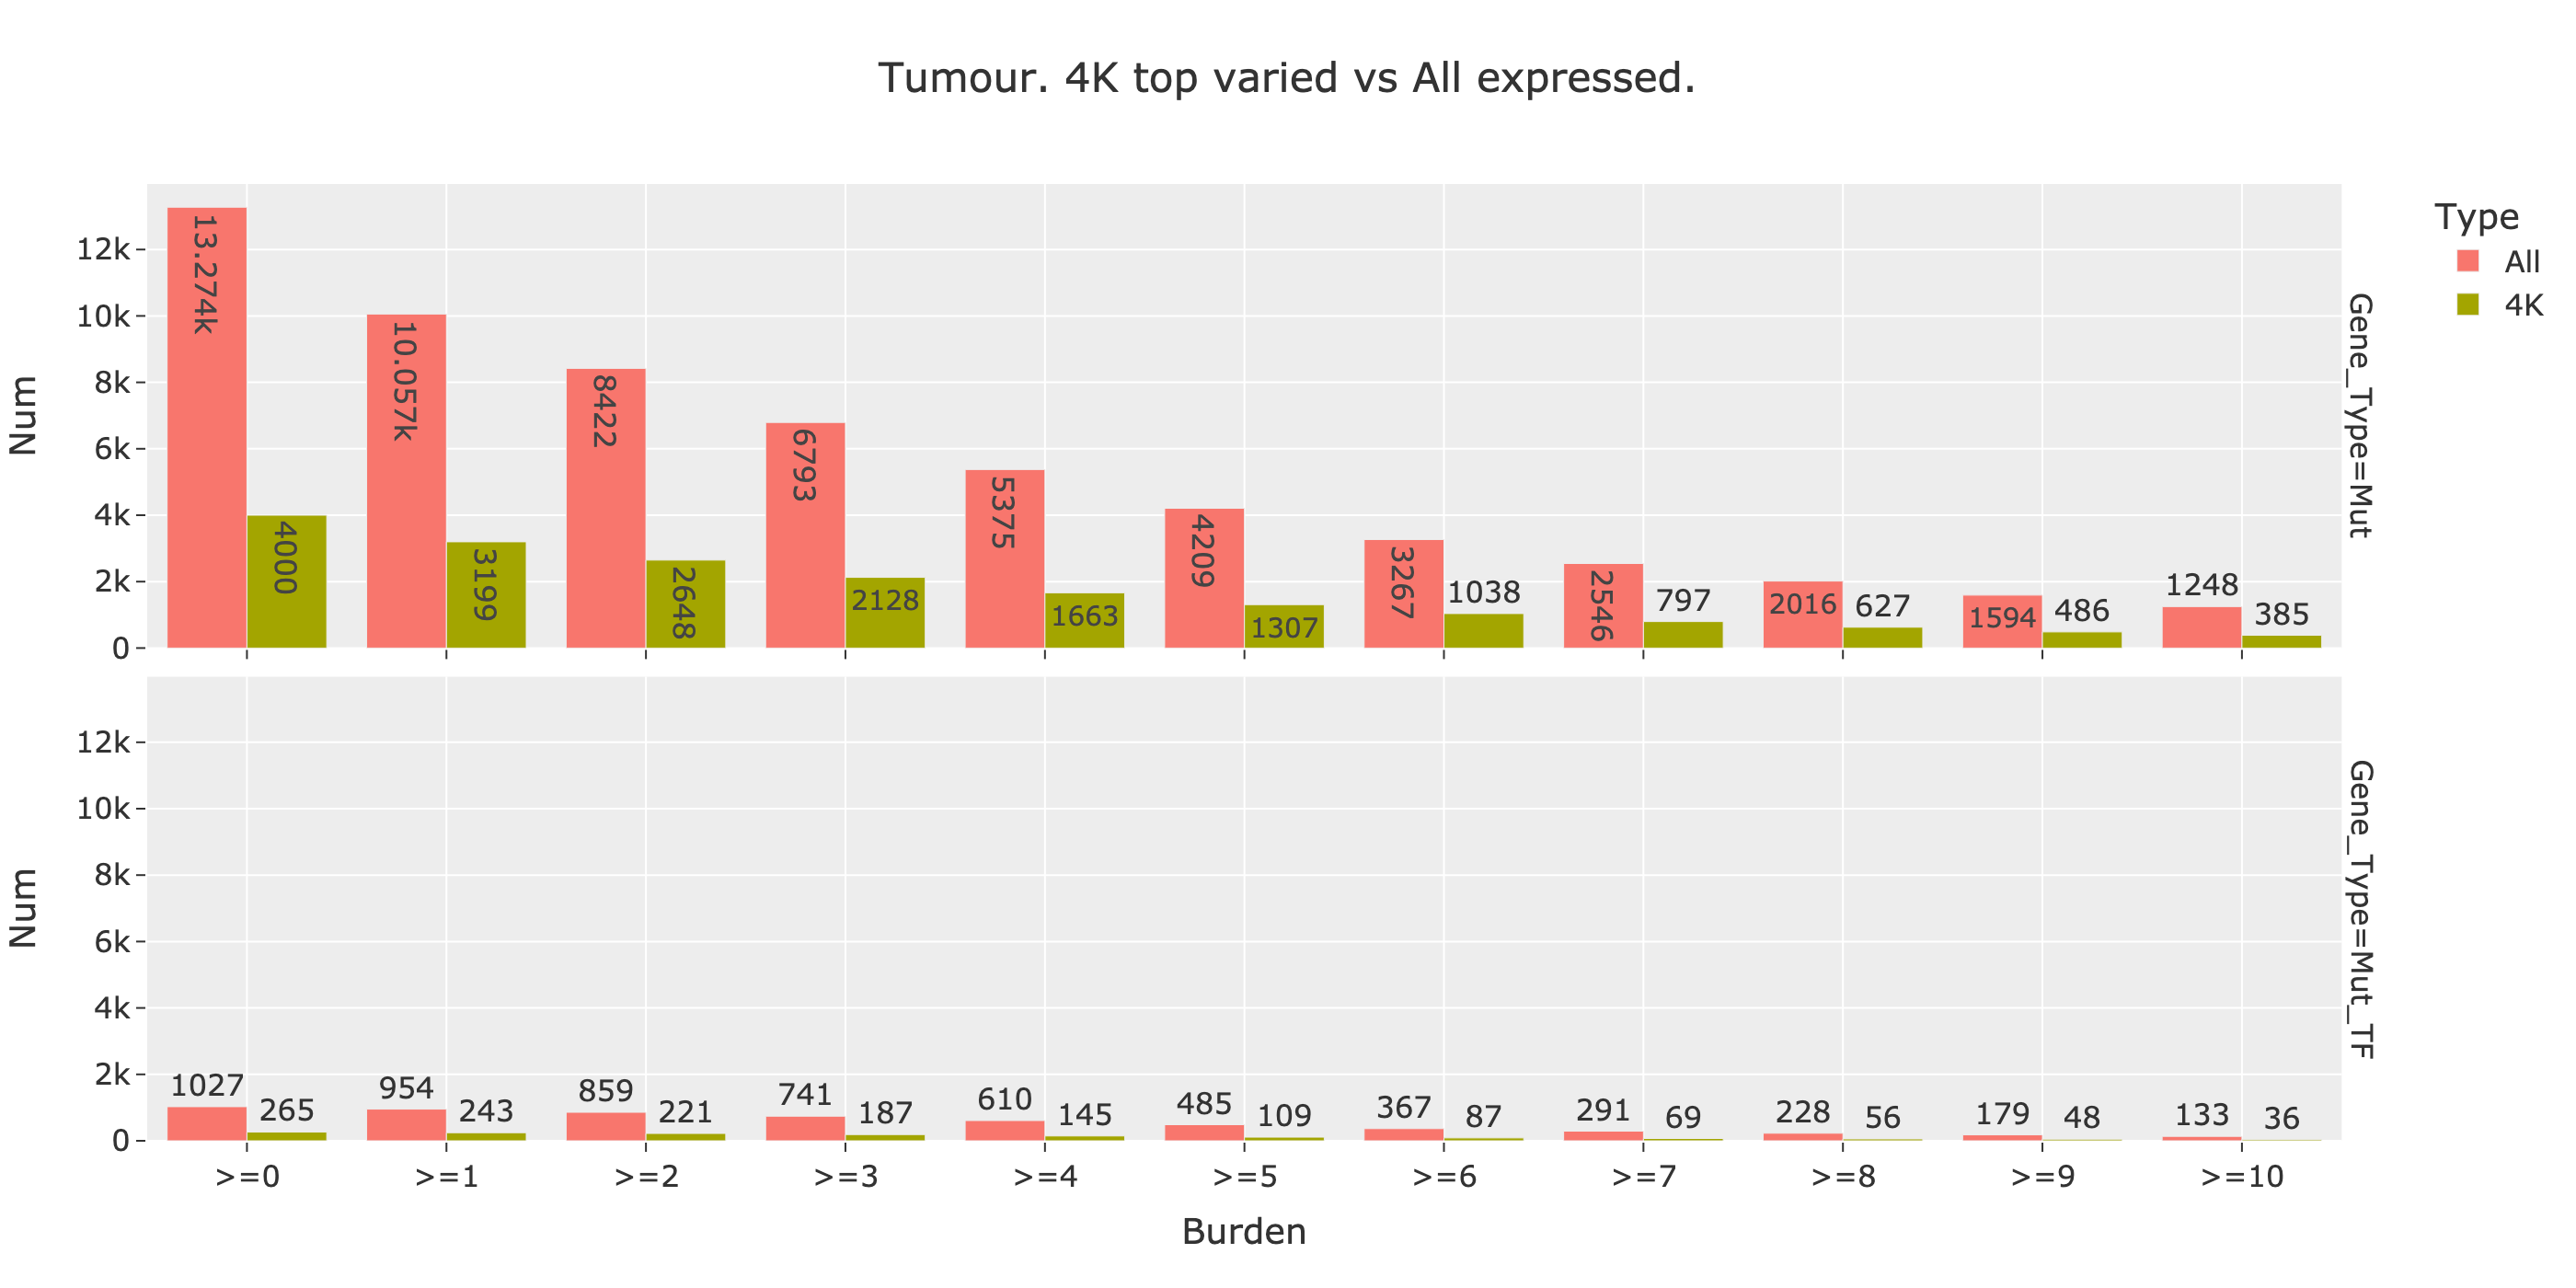
\includegraphics[width=1.0\textwidth,height=0.6\textheight,keepaspectratio]{Sections/Network_I/Resources/Tum_network/MutTF_representation_4K-all.png}
    \caption{Mutation representation in the 4K most varied genes vs all the genes expressed.}
    \label{fig:N_I:mut_rep_tum}
\end{figure}


\newpage

Structure:
\begin{todolist}
    \item [\done] Describe weight modifiers and the motivation behind them
    \item [\done] Describe how ModCon was adapted and Spearman Correlation process 
    \item [\done] Network stats - between the 3 different types of modifiers. What shall we do?
    \item Looking at the mutation representation 
    \item Leiden Community detection
    \item Sankey comparison
    \item Community comparison 
\end{todolist}


Results/figures/stats:
\begin{itemize}

    \item How the different parameters affect the network stats , thus helping to find the best network configuration. Ideally, it should be a systematic approach analysing networks with different parameters. However, I’m afraid that this will lead to a lot of data generated with little value added as there is no clear score that tells us how well a network performs on subtyping.
    \item Network stats will come in the form of distributions of the nodes value for: degree, hub score, Integrated value of Influence, weight distributions etc...
          \begin{itemize}
              \item Different network sizes. Range: 3000-10000, step 1000
              \item Edges per node for normal genes. Range: 3-10, step 10
              \item Edges per node for Transcription Factors. Range: 10-100, step 10
          \end{itemize}
    \item For a selected network include the full visualisations:
          \begin{itemize}
              \item Network in Gephi
              \item Stats of the network – Figure 7
              \item Clustering of the Module Evaluation Value (MEV)
          \end{itemize}

    \item The selected experiment I will compare it with our previous approach and the other classification such as TCGA, consensus, Lund – See an example in Figure 8
\end{itemize}


Ideally, the selection of networks should be based on the network stats, choosing the graphs that are the least nosy but also retain biological information. In practice, I'm not sure how we can do this with the current network stats, and I need to investigate/think about this more. Nevertheless, I should select two networks one for each dataset:
\begin{itemize}
    \item TCGA: very likely that I will choose with the following properties: 4000 genes, 3 edges per (normal) gene, 50 edges per (Transcription Factor)
    \item Combined TCGA and P0: Probably like the above.
\end{itemize}